% !TeX spellcheck = en_US
\documentclass[french]{yLectureNote}

\title{Mécanique du solide}
\subtitle{Physique}
\author{Paulhenry Saux}
\date{\today}
\yLanguage{Français}

\professor{F.Pettinari}
\usepackage{graphicx}%----pour mettre des images
\usepackage[utf8]{inputenc}%---encodage
\usepackage{geometry}%---pour modifier les tailles et mettre a4paper
%\usepackage{awesomebox}%---pour les boites d'exercices, de pbq et de croquis ---d\'esactiv\'e pour les TP de PC
\usepackage{tikz}%---pour deiffner + d\'ependance de chemfig
% \usepackage{tabularx}%---pour dimensionner automatiquement les tableaux avec variable X
\usepackage{awesomebox}%---Pour les boites info, danger et autres
\usepackage{menukeys}%---Pour deiffner les touches de Calculatrice
\usepackage{fancyhdr}%---pour les en-t\^ete personnalis\'ees
\usepackage{blindtext}%---pour les liens
\usepackage{hyperref}%---pour les liens (\`a mettre en dernier)
\usepackage{caption}%---pour la francisation de la l\'egende table vers Tableau
\usepackage{pifont}
\usepackage{array}%---pour les tableaux
\usepackage{lipsum}
\usepackage{yFlatTable}
\usepackage{multicol}
\newcommand{\Lim}[1]{\lim\limits_{\substack{#1}}\:}
\renewcommand{\vec}{\overrightarrow}
\newcommand{\N}[0]{\mathbb{N}}
\newcommand{\dd}{\mathrm{d}}
\newcommand{\norm}[1]{||\vec{#1}||}
\newcommand{\fo}{\psi(\vec{r},t)}
\newcommand{\foe}{\psi(\vec{r},t)\*}
\newcommand{\HH}{\hat{H}}
\newcommand{\hb}{\hbar}
\newcommand{\lap}{\nabla^2}
\newcommand{\lapcc}{\frac{\partial^2 }{\partial x^2}+\frac{\partial^2 }{\partial y^2}+\frac{\partial^2 }{\partial z^2}}
\begin{document}
\chapter{Cinématique du solide}
\section{Disque tournant}
Dans le cas d'un disque tournant, le vecteur rotation est \(\dot{\alpha}\vec{e_z}\) et si l'angle est dans le sens anti-horaire, on a \(-\dot{\alpha}\vec{e_z}\)

D'après la formule de varignon, on a \(\vec{a} = \vec{o}+\vec{AO}\wedge \vec{\Omega} = \vec{0}\). Dans le premier cas, en se plaçant en coordonnées polaires on a \(\vec{v_a} = \dot{\alpha}\vec{e_z}\wedge \rho\vec{e_{\rho}} = \dot{\alpha}\rho \vec{e_{\varphi}}\). Dans le deuxième cas, on a \(-\dot{\alpha}\rho \vec{e_{\varphi}} =+-\dot{\alpha}\rho \vec{e_{\varphi'}}\)

Si les 2 vitesses sont positives, le vecteur tourne bien dans le sens de l'angle orienté.
\section{Point sur le périmètre du disque}
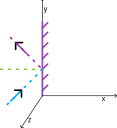
\includegraphics[scale=0.5]{methode-1}
\checkInfo{Contexte}{Un disque de rayon r tourne uniformément autour de son axe, à une vitesse angulaire \(\omega\). Son centre C
se déplace sur la droite horizontale z = r du plan vertical (Oxz) du référentiel R. On
désigne par \(\theta\) l’angle que fait un rayon avec l'axe (Cz) du disque, A étant un point quelconque situé
à la périphérie du disque et repéré par cet angle. La vitesse du centre C du disque par rapport à R est \(r\dot{\theta}\vec{e_x}\).}
 L'objectif est de trouver l'expression de \(\vec{v_a}\).

On applique Varignon :
\begin{flalign*}
\vec{v_a} &= \vec{v_c}+\vec{AC}\wedge \vec{\omega}\\
&= r\dot{\theta}\vec{e_x}-r\vec{e_{\rho}}\wedge \vec{e_y}\\
&= r\dot{\theta}\vec{e_x}+r\dot{\theta}\vec{e_{\theta}}
\end{flalign*}
On peut laisser le résultat dans la base.

Pour trouver la vitesse en \(\theta = \pi\), on exprime le vecteur en fonction de l'angle.



On trouve une vitesse nulle car la vitesse du centre de masse a été choisie pour. On retrouve donc la condition de roulement sans glissement.
\section{Différentiel d'une automobile}
\checkInfo{Contexte}{Le bati du différentiel, auquel est fixé le disque S tourne à la vitesse angulaire constante \(\omega\) autour de l’axe Oy du repère R.

Le satellite, de rayon \(a = SI_1 = SI_2\) et de centre S, peut par ailleurs tourner autour de son axe (Oz’) tout
en restant en contact avec les deux disques identiques \(P_1\) et \(P_2\) – les planétaires – de rayon \(b = HI_1 =
KI_2\). On note \(w_0, w_1, w_2\) les vitesses angulaires de rotation de S, \(P_1\) et \(P_2\) autour de leurs axes respectifs.}

On représente la situation sur cette figure :

\includegraphics[scale=0.5]{methode-2}


Les seuls degrés de liberté du système sont \(\omega, \omega_1,\omega_2,\omega_0\).

On cherche d'abord la vitesse du disque S par rapport à R.

On sait que le disque S tourne autour de l'axe y à une distance b de l'axe et à une vitesse \(\omega\). On peut donc écrire
\explanation{1}{On a choisit de fixer \(\omega\) dans le sens trigonométrique autour de \(y\), donc il est positif.}
\explanation{2}{On rappelle que dans une BOND, \(\vec{e_z}\wedge \vec{e_y} = -\vec{e_x}\)}
\begin{flalign*}
\vec{v_S} &= \vec{v_O} + \vec{SO}\wedge \vec{\omega}\\
&= \vec{0} -b \vec{e_z'}\wedge \omega\vec{e_y'}\explain{1}{left}{0}{0.5}{×}\\
&=b\omega\vec{e_x'}\explain{2}{left}{0}{0.5}{×}
\end{flalign*}

On cherche maintenant les vitesses \(\vec{v_{i1}}, \vec{v_{i2}}\) des points appartenant au disque S.

Comme on connait désormais la vitesse de S, on peut utiliser le théorème de Varignon. On a donc
\explanation{3}{Attention. Le vecteur rotation du disque S est la somme du vecteur rotation lié à sa rotation autour de l'axe y et du vecteur lié à sa rotation autour de lui-m\^eme !}
\explanation{4}{Bien que la base ne soit pas fixe, on peut quand m\^eme l'utiliser pour exprimer la vitesse}
\begin{flalign*}
\vec{v_{i1}} &= \vec{v_S} + \vec{I_1S}\wedge \vec{\Omega_S}\\
&= b\omega \vec{e_x'} + a\vec{e_y'}\wedge (\omega_0\vec{e_z'}+\omega\vec{e_y'})\explain{3}{right}{0}{0.5}{×}\\
&= (b\omega + a\omega_0)\vec{e_x'}\explain{4}{right}{0}{0.5}{×}
\end{flalign*}
Pour \(\vec{V_{I2}}\), c'est le m\^eme principe
\begin{flalign*}
\vec{v_{i2}} &= \vec{v_S} + \vec{I_2S}\wedge \vec{\Omega_S}\\
&= b\omega \vec{e_x'} -a\vec{e_y'}\wedge (\omega_0\vec{e_z'}+\omega\vec{e_y'})\\
&= (b\omega - a\omega_0)\vec{e_x'}
\end{flalign*}
On peut maintenant trouver des relations entre les \(\omega\) grace à la condition de roulement sans glissement.
Prenons d'abord \(P_1\). Soit \(I_{1,p}\in P, I_{1,s}\in S\). On sait par la condition de roulement sans glissement que :
\begin{flalign*}
\vec{v_{I_{1,s}}} &= \vec{v_{I_{1,p}}} \\
&= \vec{v_{H\in P}} + \vec{I_1H}\wedge \omega_1\vec{e_y'}\\
&= \vec{0} -b\vec{e_z'} \wedge \omega_1\vec{e_y'}\\
&= +b\omega_1\vec{e_x'}\\
(b\omega + a\omega_0)\vec{e_x'} &= b\omega_1\vec{e_x'}\\
b\omega + a\omega_0 &= b\omega_1
\end{flalign*}
Prenons ensuite \(P_2\). Soit \(I_{2,p}\in P, I_{2,s}\in S\). On sait par la condition de roulement sans glissement que :
\begin{flalign*}
\vec{v_{I_{2,s}}} &= \vec{v_{I_{2,p}}}\\
&= \vec{v_{K\in P}} + \vec{I_2K}\wedge \omega_2\vec{e_y'}\\
&= \vec{0} -b\vec{e_z'} \wedge \omega_2\vec{e_y'}\\
&= +b\omega_2\vec{e_x'}\\
(b\omega - a\omega_0)\vec{e_x'} &= b\omega_2\vec{e_x'}\\
b\omega - a\omega_0 &= b\omega_2
\end{flalign*}
On  déduit des 2 résultats précédents que
\begin{flalign*}
2b\omega &= b\omega_1 + b\omega_2\\
2\omega &= \omega_1+\omega_2
\end{flalign*}
Si la voiture est en ligne droite, \(\omega_1=\omega_2\), et en conséquence, comme \(2\omega = \omega_1+\omega_2\), on a \(\omega = \omega_1=\omega_2\). On en déduit que \(\omega_0 = 0\) et que le satellite ne tourne pas sur lui-m\^eme.

En revanche si une roue est bloquée (cas extrème), on aura par exemple \(\omega_1 = 0 \Rightarrow 2\omega = \omega_2\) et \(\omega_0 = \frac{-a}{b}\omega\). En virage, \(\omega_0 \neq 0\) selon les relations précédentes.
\section{Roulement d'un bloc de pierre sur des rondins}
\includegraphics[scale=0.5]{methode-3}
\checkInfo{Contexte}{On veut reproduire une expérience d'Obélix qui pousse, \`{a} la vitesse $v = v\mathbf{e}_x$, un bloc de pierre (modélisé par un parallélépip\`{e}de) sur des rondins de bois (cylindres creux de rayon $b$) qui ne glissent ni sur le sol, ni sous la pierre.
On définit $I_1$ le point de contact d'un rondin sur le sol et $I_2$ le point de contact du rondin sous la pierre.
On désigne par $G$ le centre de masse de ce rondin. On travaille dans le référentiel terrestre supposé galiléen et les rondins de bois tournent \`{a} la vitesse angulaire $\omega\vec{e_z}$ avec $\omega$ algébrique.}

On souhaite d'abord exprimer les vitesses des points \(I_1\) et \(I_2\) appartenant au rondin de bois en fonction de la vitesse de G. On applique Varignon :
\begin{flalign*}
\vec{v_{I_1}} &= \vec{v_G} + \vec{I_1G}\wedge \omega \vec{e_z}\\
&= v_g\vec{e_x} +b\vec{e_y}\wedge \omega \vec{e_z}\\
&= v_g\vec{e_x} +b\omega\vec{e_x}\\
&= (v_g+b\omega)\vec{e_x}
\end{flalign*}
De la m\^eme façon, au point \(I_2\), on a
\begin{flalign*}
\vec{v_{I_2}} &= \vec{v_G} + \vec{I_2G}\wedge \omega \vec{e_z}\\
&= v_g\vec{e_x} -b\vec{e_y}\wedge \omega \vec{e_z}\\
&= v_g\vec{e_x} -b\omega\vec{e_x}\\
&= (v_g-b\omega)\vec{e_x}
\end{flalign*}

Exprimons maintenant les conditions de roulement sans glissement en \(I_1\) et en \(I_2\).

On a \(I_1\in \text{sol}, I_1\in \text{roue}\), avec \(\vec{v_{I_1\in \text{sol}}} = \vec{0}\). On en déduit que \(\vec{v_{I1,s}} = (v_g+b\omega)\vec{e_x} = \vec{0} \Rightarrow v_g = -\omega b\)

Pour \(I_2\), on a \(I_2\in \text{pierre}, I_2\in \text{roue}\), avec \(\vec{v_{I_2\in \text{pierre}}} = \vec{v}\) selon l'énoncé\marginTips{car solide en translation donc tous les points ont la m\^eme vitesse.} et \(\vec{v_{I_2, \text{pierre}}} = (v_g-b\omega)\vec{e_x}\). On en déduit que \(v_g-\omega b = v\).

On peut en déduire la valeur de \(v_g\). Avec les 2 conditions, on trouve que \(-2b\omega = v\), ce qui nous permet de trouver une valeur de \(\omega = \frac{-v}{2b}\)\marginCheck{Le signe de \(\omega\) est négatif, ce qui est cohérent car le rondin tourne dans le sens horaire, la pierre étant poussée vers la droite.}. En injectant cett expression dans la première condition, on trouve que \(v_g -(-\frac{v}{2b})b = \frac{v}{2}\).
 \end{document}
